\chapter{Introduction}


%%%%%%%%%%%%%%%%%%%%%%%%%%%%%%%%%%%%%%%%%%%%%%%%%%%%%%%%%%%%%%%%%%%%%%%%%%%%%%%%
\section{Research background and objective}
Recently, aerial manipulation has attracted a lot of attention in the robotic research field \cite{ollero_2021_past}. Compared with conventional ground robot manipulation, aerial manipulation emphasizes that the manipulator itself could move to places that are difficult to reach. Usually, aerial manipulation tasks need to be executed by a drone equipped with a manipulator. Current morphologies include attaching a static manipulator (e.g., a tool or a stick) to the drone, mounting a serial robotic arm or a parallel delta arm on the drone. In all cases, the system can be considered as consisting of two parts: the drone itself and the manipulator. The drone part is used for locomotion and the manipulator part used for manipulation. Such principle of designing has proven effective across various tasks. However, they all suffer from certain issues to varying degrees.

On the other hand, one of the newest aerial robots for aerial manipulation is the multi-link aerial robots. Multi-link aerial robots are capable of actively deforming their articulated serial-link structures in the air, and this deformability provides additional degrees of freedom for manipulation during flight \cite{zhao_2021_singularity, zhao_2018_design, yang_2018_lasdra, hameed_2025_dragonfly}. Its structure is designed to go through narrow space or enhance the operation wrench \cite{zhao_2020_online, zhao_2022_forceful}. Owing to these structural advantages, multi-link aerial robots offer opportunities for applications, including inspection and search-and-rescue tasks. Their effectiveness has been demonstrated in a variety of experimental tasks, such as grasping objects \cite{hameed_2025_dragonfly, shi_2020_aerial, zhao_2023_versatile}, opening sliding door \cite{sugito_2022_aerial} and manipulating valves \cite{zhao_2022_forceful}.

However, when facing a broader range of aerial manipulation tasks, conventional aerial manipulation systems are often insufficient. A representative interaction scenario is a contact-rich surface sliding task, in which an aerial robot is typically required to maintain a pressing contact between its end-effector and an unknown uneven surface while following a desired sliding trajectory \cite{bodie_2020_active, trujillo_2019_novel, tognon_2019_truly}. Such tasks inherently involve a coupling between unmodeled surface geometry and frictional effects, leading to significant uncertainties in both the external wrench and the contact geometry experienced by the robot. Additionally, in practical aerial applications such as bridge inspection and infrastructure maintenance, extra task-relevant structures on the robot may also be required to perform specific trajectory. For example, cameras mounted on the aerial platform may need to take video in a desired viewpoint, while power cable or sensors attach on the aerial platform may also need to preserve a specific position. Therefore, as the contact interaction situation varies during surface sliding, these position requirements are also needed to be considered by changing the configuration of the multi-link structure through requirements of tasks and external geometric disturbance. 

As a result, the controller must exhibit both robustness and compliant behavior, enabling the end-effector to remain resilient to force disturbances while the relative configuration adaptation to changing contact conditions. Nevertheless, existing control methods for multi-link aerial robots remain limited in achieving this unified combination of robustness and compliant interaction \cite{ollero_2021_past}.  This limitation primarily stems from their lack of perception of external conditions, which prevents the controller from adapting its force and motion responses to uncertainties in the external wrench and contact conditions.


% (it is essential to further address more complex interaction scenarios that involve sustained contact and environmental uncertainties.)

\begin{figure}[t]
  \centering
  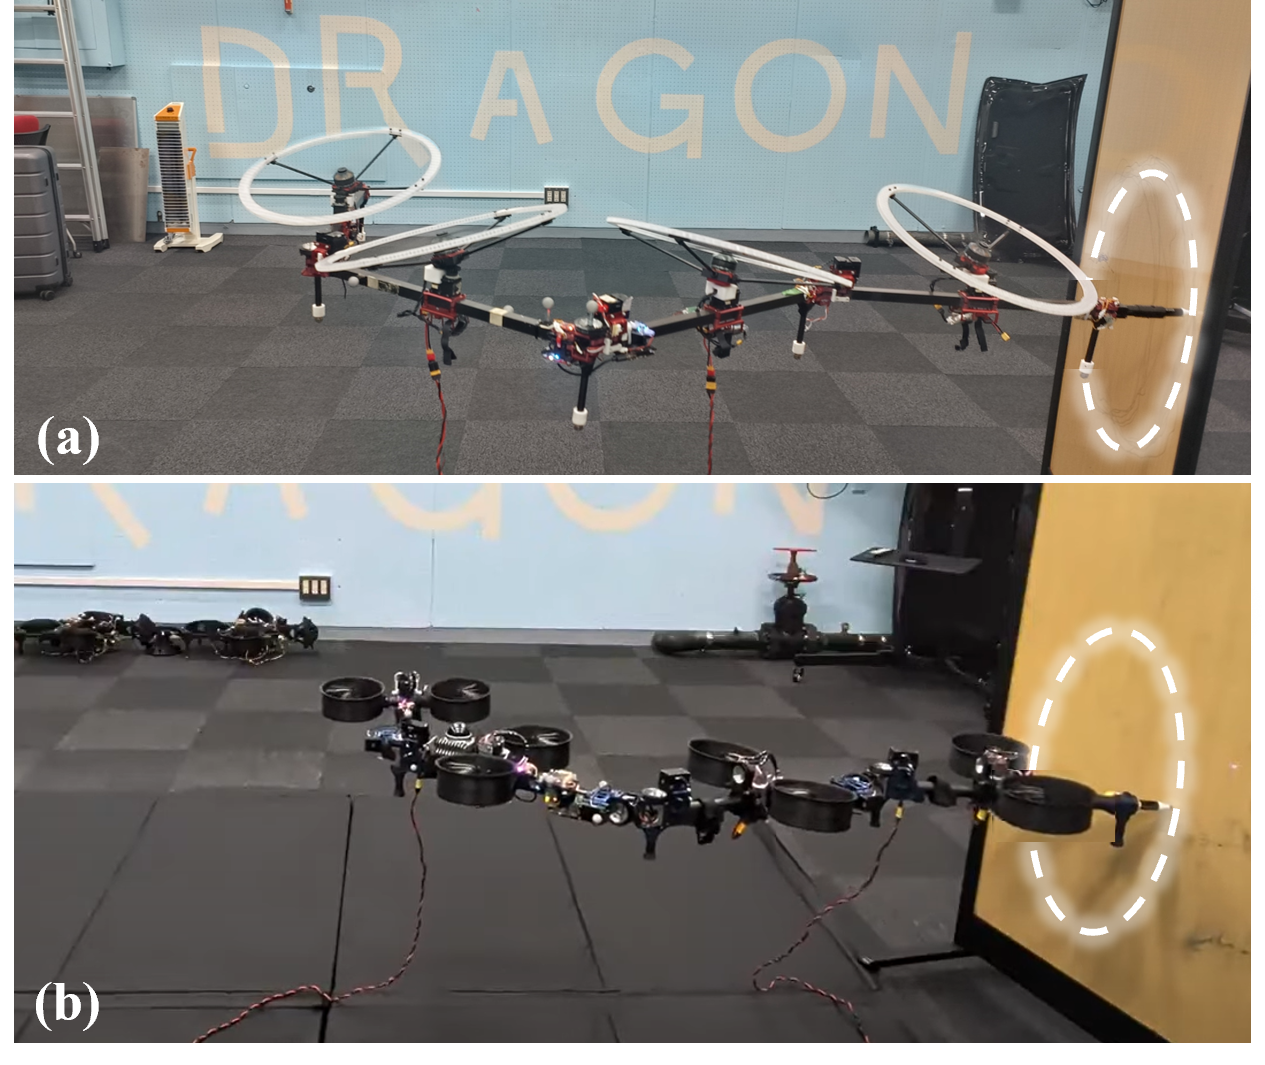
\includegraphics[width=\linewidth]{figures/chapter1/main_figure.png}
  \caption{A multi-link aerial robot is tracking a circular trajectory on a sloped board while maintaining contact. The desired trajectory is marked by a white dashed line. (a) Side view. (b) Top view.}
  \label{fig:main_figure}
  \vspace{-7mm}
\end{figure}

To execute tasks in such kind of interaction scenarios, previous work has commonly adopted force-control strategies such as impedance control and admittance control \cite{ollero_2021_past}. However, they each have their own advantages and disadvantages. Impedance control performs well in regulating interaction forces and resisting external force disturbances, but typically exhibits limited adaptability to changing contact geometry. In contrast, admittance control is effective in adapting to geometric variations, but is generally less robust against large interaction force disturbances. These differences originate from the complementary yet opposite causal relationships of impedance and admittance control paradigms \cite{ott_2010_unified}. Consequently, contact-rich tasks that simultaneously require disturbance rejection and adaptation to uncertain surface geometry cannot be reliably addressed by either approach alone, naturally motivating a combination of both control principles to achieve resilient and adaptive interaction capabilities.

Previous researches have pay a lot of attentions on impedance control or admittance control on aerial robot. However, currently, there is not a control method combined them together, while obviously we need both of their abilities. This is because achieving such a combination is not trivial. Due to the opposite causality of impedance and admittance control, a single actuation source cannot independently realize both interaction objectives and generally requires additional coordination mechanisms \cite{ott_2010_unified}. Conventional aerial robot platforms, which rely exclusively on rotor thrusts, inherently possess only a single actuation source and are therefore limited in their ability to simultaneously exploit the complementary properties of the two paradigms.


Luckily, if the aerial robot is mounting a robotic arm or is a multi-link aerial robot, this problem can be solved. The current situation is, although some aerial manipulation platforms (e.g., \cite{lippiello_2012_cartesian, cataldi_2016_impedance}) introduce joint actuation and therefore provide additional actuation source, existing studies have not leveraged this structural characteristic to simultaneously employ both impedance and admittance control. This limitation further motivates the design of our control strategy. Considering the future scalability of this control framework, we chose to use the multi-link aerial robots as the development platform, and combine impedance and admittance control simultaneously.

In this work, we propose a novel hybrid impedance--admittance control enabled by multi-link aerial robots, which exploits the two independent actuation sources of the robot by assigning them distinct control roles. In particular, rotor thrusts govern the global motion of the platform, whereas the joint actuators regulate the end-effector pose relative to the platform's body. This structure enables impedance control to be implemented through rotor thrusts and admittance control through joint actuation, allowing both paradigms to be realized simultaneously on a single aerial platform. Within the proposed framework, impedance control regulates the aerial robot's center-of-gravity (CoG) motion to achieve disturbance-resilient interaction, while admittance control adjusts joint angles to accommodate unmodeled surface geometric and contact-induced variations. Through this division of roles, the proposed strategy enables resilient and adaptive sliding along unknown surfaces. The task execution process is illustrated in Fig.~\ref{fig:main_figure}.


%%%%%%%%%%%%%%%%%%%%%%%%%%%%%%%%%%%%%%%%%%%%%%%%%%%%%%%%%%%%%%%%%%%%%%%%%%%%%%%%
\section{Previous Research}

\subsection{Morphologies of aerial robot for aerial manipulation}
% Considering that the aeria manipulation is directly derived from the ground manipulation field, the morphology of the manipulatiors attached in the aerial robot is usually very similar with those in the ground robot. Obviously, we can used the mechanical design and control method that have been demonstrated in the ground robot field.
%The morphology is very important for the aerial manipulation\cite{ollero_2021_past}. 
We can briefly divide the morphologies of aerial manipulation into four types: single rigid body morphology, parallel morphology, series morphology and other specific morphology like multi-link aerial robot as illustrated in Fig.~\ref{fig:morphologies}. These morphologies have their own features for different type of tasks.

The single rigid body morphology is just install a rod or a stick on the aerial robot, and the manipulator usually keeps static to the aerial robot. This kind of morphology is very simple, we don't need to think about how to control the end effector itself. 
By mainly controling the aerial robot itself to provide degree of freedom for the end effector, the rigid manipulator is used for task like push-and-slide and peg-in-hole. 
%The end effector is usually a pad that installed with sensors, or a roller to move in the surface %smoothly. 
The main requirement is the pose of manipulator, and it is ragulate by aerial robot's pose.
In the recent research. For example Bodie et al. \cite{bodie_2020_active} uses a static end effector to inspect bridge. Brunner et al. \cite{brunner_2022_planning} realized to operate an articulated door. 
%Actually, they did not use the manipulator it self to do the tasks.
However, for more complicated tasks, the rigid manipulator may be not enough. Meanwhile, the rigid manipulator do not have extra d.o.f, so if the requirements need more, this type is not good. 


The parallel morphology is defined as an aerial robot mounted with a delta manipulator. Since the delta manipulator has the adventages of low inertia, high stiffness and fast response due to its mechnical structure, the paraller morphology can realize high-speed motion and accurate position control. 
Due to these adventages, a few researchers have used such kind of morphology. Guo et al. \cite{guo_2024_flying} performed calligraph on a board with the parallel morphology,showing the potential of this morphology for precise manipulation tasks.Deng et al. \cite{deng_2025_whole} realized high speed manipulation like push objects and grasping object, indicating the ability of achieve fast motion requirements.
The above application demonstrate that the parallel morphology can perform well in high precision and high speed requirements. However, since the surface sliding tasks usually requires large work space that the delta manipulator do not have, this morphology will struggle when faced with a wider range of surface geometry variations.

\begin{figure}[t]
  \centering
  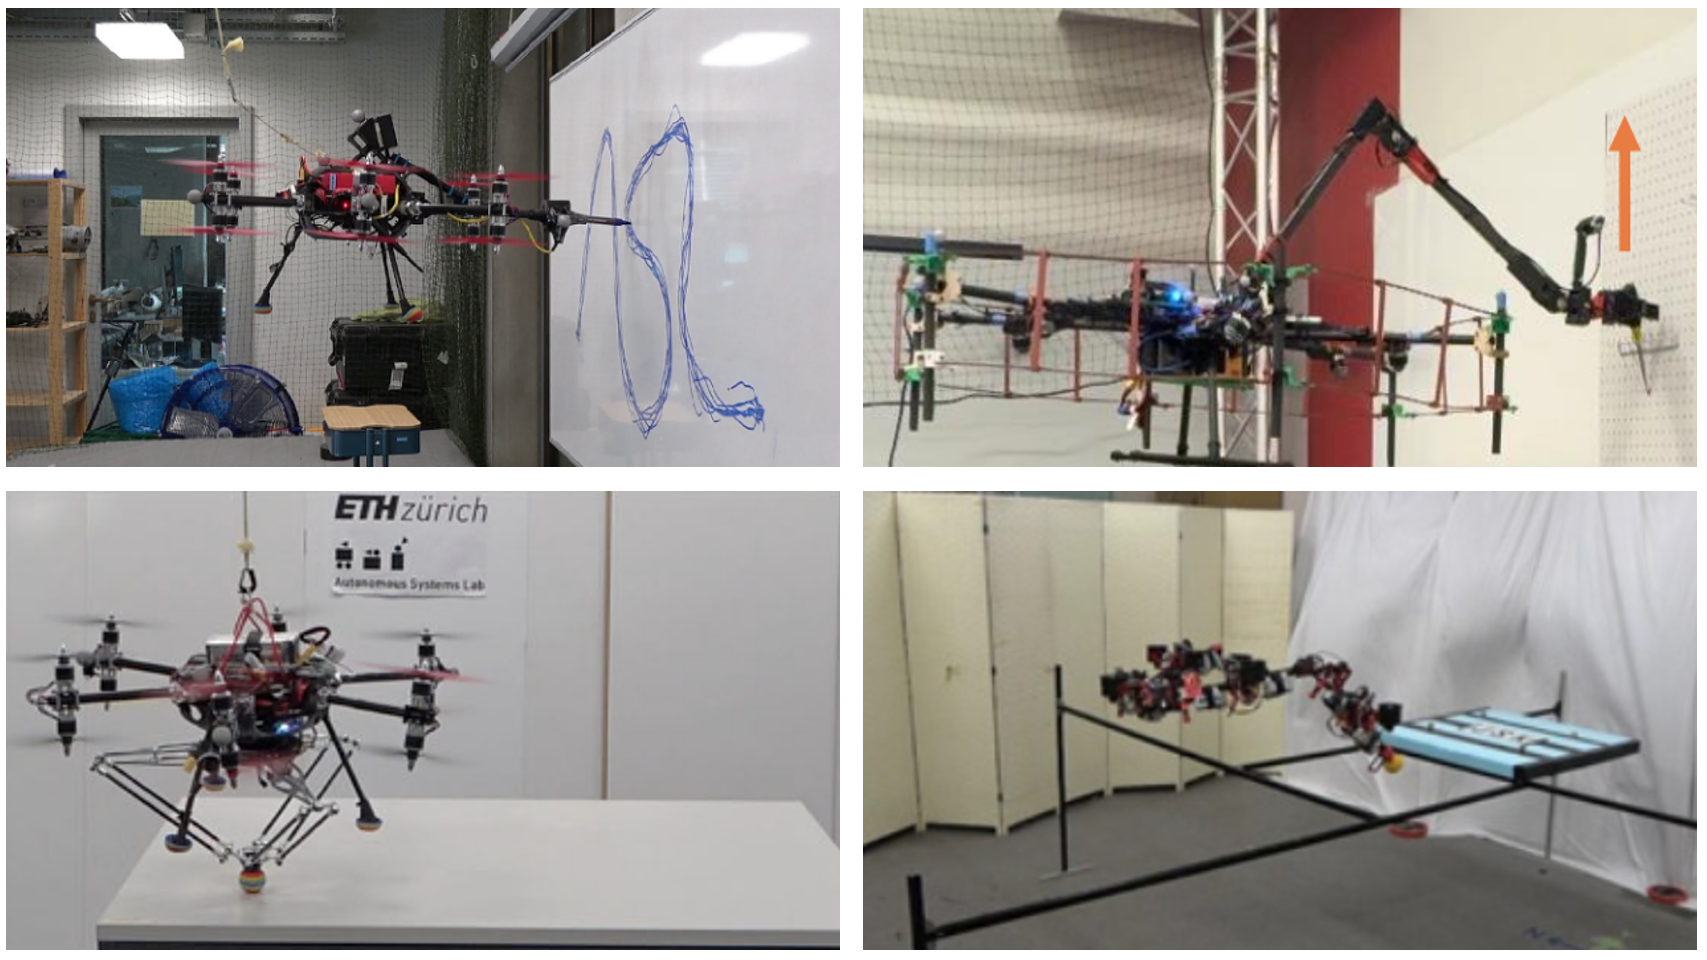
\includegraphics[width=\linewidth]{figures/chapter1/morphologies.png}
  \caption{Four morphologies of aerial robots. (a) Static end effector. (b) serial manipulator. (c) delta manipulator. (d) multi-link aerial robot}
  \label{fig:morphologies}
  \vspace{-7mm}
\end{figure}

The serial morphology is defined as an robotic arm manipulator mounted on an aerial robot. The serial structures of robotic arm provides large work space. In contrast to the parallel morphology, the serial morphology is usually used in tasks requiring large working space and obstacle avoidance ability. 
Move a robotic arm to an aerial robot is an intuitive idea, therefore a lot of researches realize it. He et al. \cite{he_2025_flying} used serial arm to draw a relative large figure on a board. 
Lee et al. \cite{lee_2025_autonomous} realized SE(3) operation like peg-in-hole in a large scenario. 
Both demonstrated that the serial morphology possesses strong operational capabilities and potential.
Due to the multi-DOF structure, both serial morphology and multi-link morphology provide flexible manipulation capabilities for aerial robots.


%Too support the hole arm, it needs high quality rotor, which will also bring high weight.

The mutli-link aerial robot itself can be called multi-link morphology. This type of morphology can be regarded as a flying robotic arm, so it has all the strengths of serial morphology. Meanwhile, the multi-link aerial robot can trans trought narrow gap that the normal aerial robot can not achieve.
The extra d.o.f of multi-link aerial robot can also help it do more things. Sugito et al. \cite{sugito_2022_aerial} used multi-link aerial robot to push a door. Shi et al. \cite{shi_2020_aerial} used multi-link aerial robot to grasp a box. We already know the morphology with serial structures has the ability in surface sliding tasks. However until now, the multi-link aerial robot has not been used in the surface sliding tasks. THerefore in this work, considering the morphology features, we develop the control framework for the multi-link aerial robot.


In conclusion, the morphologies of aerial robots would influence the abilities: parallel robotic arms usually used for agile manipulation tasks, while the series arms are used for large working space tasks. When it comes to complicated aerial manipulation tasks like surface sliding tasks, multi-link aerial robot is a good choice.




\subsection{control method used in aerial manipulation}
For more and more interaction aerial manipulation tasks, it is important to introduce force-control methods. Previous work has commonly adopted force-control strategies such as impedance control and admittance control \cite{ollero_2021_past}. 

Both impedance and admittance control can be considered as can be considered as general impedance control \cite{valency_2003_accuracy}. The concept of impedance control is put forward by Hogan \cite{hogan_1984_impedance}. In his paper, the environment should be considered as an admittance, therefore if the robot performs like an impedance, the power flow will be reasonable. Currently, the conception of impedance and admittance controller becomes a little different. If the system perform like a compliant second order system, it can be called as impedance control. In detail, the impedance control wishes the system performs like a real second order system, the main idea of it is to design a second order system. On the other hand, the admittance control tries to imitate a second order system, whose position almost follow the design system. Transparently, both impedance and admittance control performs similarly, but their causalities are completely opposite. Due to their concern object, The impedance control is better used in the force control actuator, and the admittance control has better used in position control actuator, or perform as a filter to provide reference position command for lower layer controllers.

Among these strategies, impedance control has been extensively explored for aerial robots. 
For the beginning of aerial manipulation research, the impedance control method was used \cite{ollero_2021_past}.
Forte et al. \cite{forte_2012_impedance} calculated the 3D impedance control for a single rigid body aerial robot, and Lippiello et al. \cite{lippiello_2012_cartesian} put forward the impedance equation of an aerial robot with a serial arm. In his paper, the aerial robot itself and the 3-dof robotic arm is set different dynamic parameters, which also gives this thesis inspiration. After those work introduce impedance control into aerial manipulation tasks, the community more focused on the effect impedance control can realize.
In recent years, the impedance control has been used in more complicated tasks.
Bodie et al. \cite{bodie_2020_active} introduced a six-DOF axis-selective impedance controller capable of adjusting impedance gains based on surface proximity. In this work, the impedance control is considered as the adjusting part. This work realized sliding on the surface, following a specific trajectory, which can be used for bridge inspection task.
Zhang et al. \cite{zhang_2022_learning} employed learning-based techniques to adapt the impedance parameters, which helps the aerial robot sliding on an uneven plane. Both work pay attention to use impedance control as a adjusting part to adapt to the unknown external environment that has different force requirements. 
We can see that using impedance control in aerial robot is relatively mature. However, current literatures are mainly focusing on designing a useful control framework instead analyzing how the impedance controller perform in different tasks, or analyzing how the parameters effect the performance of aerial manipulation.
These methods can effectively respond to external force disturbances through gain modulation. However, there is limited evidence that they remain effective in environments with uneven or irregular surfaces by adapt to the geometric variations. 

In addition to impedance approaches, admittance control has also been applied in aerial manipulation tasks. 
Someone uses admittance control as a filter, and the framework use PID control as the inner controller.
Ryll et al. \cite{ryll_2019_6d} enabled an aerial robot to follow variations in the contact-plane geometry, yet the induced lateral force disturbances caused noticeable rotational deviations.
Cataldi et al. \cite{cataldi_2016_impedance} used an admittance filter to calculate the reference values.

The admittance control is less than impedance control.

In our framework ,admittance control is more like controlling a robotic arm instead of an aerial robot. Therefore, we will introduce admittance control used in controlling robotic arms. 
Admittance control has been used in robotics arm like




In conclusion, while these studies demonstrate the potential of impedance- or admittance-based approaches for aerial manipulation tasks in interaction scenarios, each method inevitably inherits the limitations of its underlying control principle.
This thesis tries to combine these two controllers together on the same platform in order to gain both of their strengths.
\subsection{cooperative aerial manipulation}
In the surface sliding task, besides the contact requirements, there must be some secondary task, such as taking photos or keep the cable stable. This kind of requirements are not the essential problem in surface sliding, but it will effect whether we can use the whole system into the real application. In this thesis, we can also answer how to use the multi-link structure to achieve the secondary requirements.

A similar solution for the secondary requirements is the cooperative aerial manipulation. In this kind of aerial manipulation, multi aerial robots can take part in the task and be respond to some requirements. The cooperative aerial manipulation can be divided into two types. First is all of the aerial robots share the some ability, like two aerial robot work together to grasp a long stick. Second is the aerial robots have different requirements. We can image a dual aerial robots system with a prior robot and a secondary robot, the prior robot need to completed the contact tasks, and the secondary robot help it in photography. Transparently, the secondary aerial robot also has special control requirements, so we can use the method in the first type, for example to image a virtual stick between the contact point and the photography point, and these two aerial robots need to grasp the virtual stick. By using the same control method, these type of cooperative aerial manipulation tasks can also be solved. So in our view, to solve the secondary requirements, we must research for the cooperative aerial manipulation.

Most of the cooperative aerial manipulation pay attention to two aerial robots. The fundamental of the cooperative aerial manipulation is to control two frames trajectories simultaneously. Our multi-link aerial robot can also do that by using its two ends. Additionally, the double aerial robots manipulation must has problems like: the two robots need to wireless connect to transport the information. Meanwhile, the two ends of multi-link aerial robot is connected by physical structures, which must be more reliable compared to the double aerial robot system.

Caccavale et al. \cite{caccavale_2015_cooperative} tried to used impedance control to adjust two aerial robots in order to grasp a stick. We can imitate it.

%%%%%%%%%%%%%%%%%%%%%%%%%%%%%%%%%%%%%%%%%%%%%%%%%%%%%%%%%%%%%%%%%%%%%%%%%%%%%%%%
\section{The construction of the thesis}

This thesis investigates the force control method of multi-link aerial robot. The overall structure of the thesis is organized as follows.


\begin{itemize}
	\item Chapter 1 introduces the research background and motivation of this study, reviews related work about morphologies of aerial robots, force control methods used in aerial manipulation, and the current situation of cooperative aerial manipulation. Based on above discussion, the motivation, objectives and contributions of this thesis are introduced.
	\item Chapter 2 presents the mechanical design of two different types of multi-link aerial robots. The modeling process is introduced.
	\item Chapter 3 introduces the basic concepts of impedance control and admittance control, analyzes how the impedance control can redesign the dynamic parameters of a system, and how the admittance influence the distance between the CoG and the end effector. The effects of the hybrid controller is proved on the 2D multi-link aerial robot platform Hydrus Xi.
	\item Chapter 4 introduces how to combined impedance control and admittance control together on the same system. The admittance control is used for adjust the internal configuration of the aerial robot, while perform adaptation to the external geometric variations. The effects of the intergrated hybrid controller is proved on the 3D multi-link aerial robot platform DRAGON.
	\item Chapter 5 presents experimental results.
	\item Finally, Chapter 6 concludes the thesis by summarizing the main findings and contributions of this work and outlining directions for future research
\end{itemize}


